\chapter{Exact inference}


\section{Inference by enumeration}
\marginnote{Inference by enumeration}

Method to sum out a joint probability without explicitly representing it
by using CPT entries.

Enumeration follows a depth-first exploration and has a space complexity of $O(n)$
and time complexity of $O(d^n)$.
It must be noted that some probabilities appear multiple times but 
require to be recomputed because of the definition of the algorithm.

\begin{example}[Burglary]
    Given the Bayesian network:
    \begin{center}
        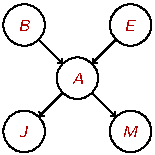
\includegraphics[width=0.15\textwidth]{img/_burglary_net.pdf}
    \end{center}
    We want to compute $\textbf{P}(B \mid j, m)$:
    \[
        \begin{split}
            \textbf{P}(B \mid j, m) &= \frac{\textbf{P}(B, j, m)}{\prob{j, m}} \\
                &= \alpha \textbf{P}(B, j, m) \\
                &= \alpha \sum_{e} \sum_{a} \textbf{P}(B, j, m, e, a) \\
                &= \alpha \sum_{e} \sum_{a} \textbf{P}(B) \prob{e} \textbf{P}(a \mid B, e) \prob{j \mid a} \prob{m \mid a} \\
                &= \alpha \textbf{P}(B) \sum_{e} \prob{e} \sum_{a} \textbf{P}(a \mid B, e) \prob{j \mid a} \prob{m \mid a} \\
        \end{split}  
    \]

    This can be represented using a tree:
    \begin{center}
        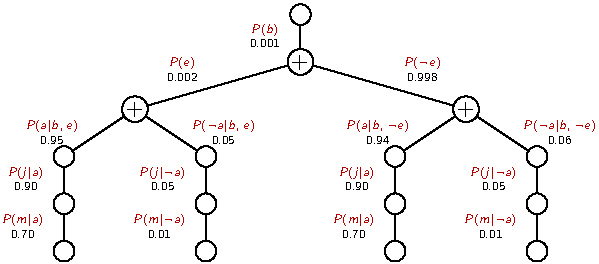
\includegraphics[width=0.75\textwidth]{img/_burglary_enumeration.pdf}
    \end{center}
\end{example}


\section{Inference by variable elimination}
\marginnote{Inference by variable elimination}
Method that carries out summations right-to-left and stores intermediate results (called factors).

\begin{description}
    \item[Pointwise product of factors] $f(X, Y) \times g(Y, Z) = p(X, Y, Z)$
        \begin{figure}[H]
            \centering
            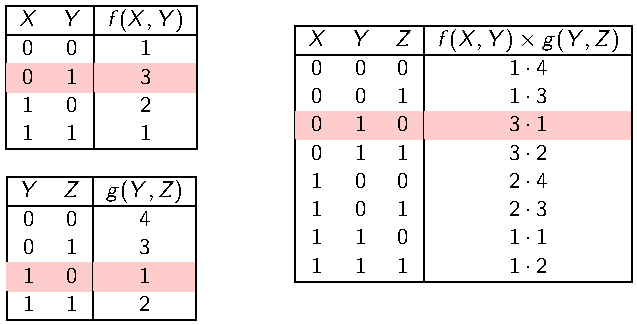
\includegraphics[width=0.5\textwidth]{img/_pointwise_factors.pdf}
            \caption{Example of pointwise product}
        \end{figure}

    \item[Summing out]
        To sum out a variable $X$ from a product of factors:
        \begin{enumerate}
            \item Move constant factors outside (i.e. factors that do not depend on $X$).
            \item Compute the pointwise product of the remaining terms.
        \end{enumerate}

        \begin{example}
            \[ 
                \begin{split}
                    \sum_X f_1 \times \dots \times f_k &= f_1 \times \dots \times f_i \sum_X f_{i+1} \times \dots \times f_k \\
                        &= f_1 \times \dots \times f_i \times f_X
                \end{split}    
            \]
        \end{example}
\end{description}

\begin{example}[Burglary]
    Given the Bayesian network:
    \begin{center}
        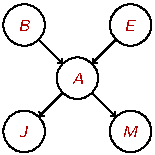
\includegraphics[width=0.15\textwidth]{img/_burglary_net.pdf}
    \end{center}
    We want to compute 
    $\textbf{P}(B \mid j, m) = \alpha \textbf{P}(B) \sum_{e} \prob{e} \sum_{a} \textbf{P}(a \mid B, e) \prob{j \mid a} \prob{m \mid a}$.
    
    We first work on the summation on $A$.
    We introduce as factors the entries of the CPT:
        \[ \textbf{P}(B \mid j, m) = \alpha \textbf{P}(B) \sum_{e} \prob{e} \sum_{a} f_A(a, b, e) f_J(a) f_M(a) \]
    Note that $j$ and $m$ are not parameters of the factors $f_J$ and $f_M$ because they are already given.
    We then sum out on $A$:
        \[ \textbf{P}(B \mid j, m) = \alpha \textbf{P}(B) \sum_{e} \prob{e} f_{AJM}(b, e) \]

    Now, we repeat the same process and sum out $E$:
        \[ \textbf{P}(B \mid j, m) = \alpha \textbf{P}(B) f_{EAJM}(b) \]

    At last, we factor $\textbf{P}(B)$:
        \[ \textbf{P}(B \mid j, m) = \alpha f_B(b) f_{EAJM}(b) \]
\end{example}


\subsection{Irrelevant variables}
\marginnote{Irrelevant variables}
A variable $X$ is irrelevant if summing over it results in a probability of $1$.

\begin{theorem}
    Given a query $X$, the evidence $\matr{E}$ and a variable $Y$:
        \[ Y \notin (\texttt{Ancestors($\{ X \}$)} \cup  \texttt{Ancestors($\matr{E}$)}) \rightarrow Y \text{ is irrelevant} \]
\end{theorem}

\begin{theorem}
    Given a query $X$, the evidence $\matr{E}$ and a variable $Y$:
    \[ Y \text{ d-separated from } X \text{ by } \matr{E} \rightarrow Y \text{ is irrelevant} \]
\end{theorem}


\subsection{Complexity}
\begin{description}
    \item[Singly connected networks] 
        Network where any two nodes are connected with at most one undirected path.
        Time and space complexity is $O(d^k n)$.
    \item[Multiply connected networks] The problem is NP-hard.
\end{description}


\section{Clustering algorithm}
\marginnote{Clustering algorithm}

Method that joins individual nodes to form clusters.
Allows to estimate the posterior probabilities for $n$ variables with complexity $O(n)$.